We investigated three versions of the AWP design described in the last section of the previous chapter. The first type we present is based on 3D printed \ce{Al2O3}, the second type is produced using ordinary 3D printed polymers and the third type consists of SLE fused silica glass waveplates as described in the previous chapter. The results are obtained through the minimization of the two objective functions defined in the previous chapter.

% This AWP type differs from the other two in the sense that the phase shift is not caused by form birefringence, but instead by intrinsic birefringence which stems from the crystallographic orientation of the material. The second type is similar to the fused silica glass AWP in the sense that it is also based on form birefringence but the structure is 3D printed by typical of the birefringence is not from the structure but instead on the crystallographic orientation of the material. 

\section{Ceramic AWP}
In a publication by Ornik et al. it was shown that \ce{Al2O3} as a 3D printed ceramic exhibited birefringent properties. A birefringence of approximately $0.05$ was reported. This value is fairly low compared to the birefringence of sapphire which is the crystalline form of \ce{Al2O3} with a birefringence of approximately $0.32$. 

\begin{figure}[ht]
    \centering
    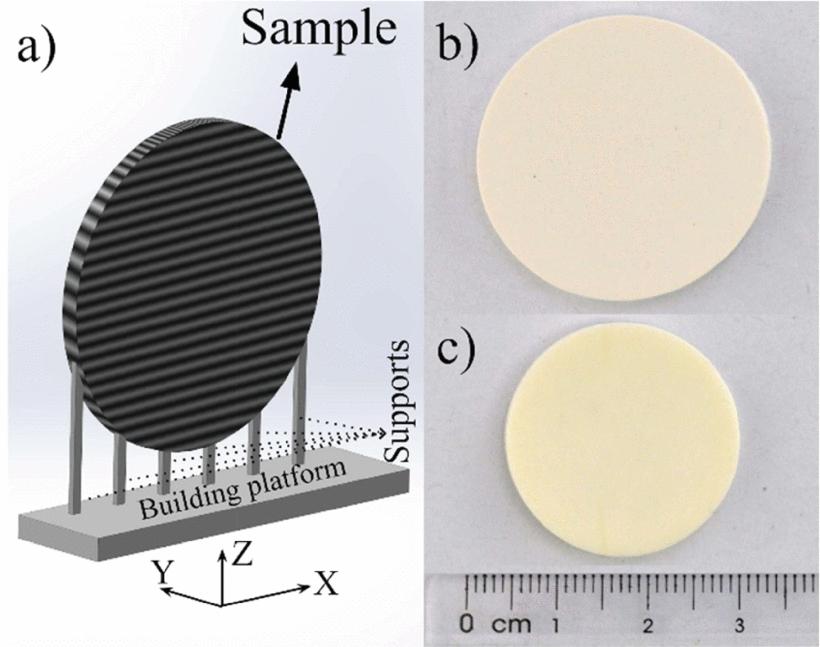
\includegraphics[scale=0.4]{images/5_chapter05/ornikabclarge.png}
    \caption{Schematic image of the a) printed sample as well as photographs of b) green and c) sintered Alumina. Source: \cite{Ornik2021}}
    \label{fig:ornik1abc}
\end{figure}
% TODO caption is copy from jan paper

It was further shown that the direction of the slow axis was parallel to the printing direction. A sketch of how the samples are printed is shown to the left in figure \ref{fig:ornik1abc}, where the arrow indicates the printing direction. The top right side shows an actual image of the green sample and the bottom right shows an image of the sample after sintering. For the sintering step the sample is slowly heated to \SI{1700}{\celsius} which causes it to shrink, in this case by around \SI{21}{\volpercent}. In total two different samples were characterized and the result of this characterization is shown in figure \ref{fig:ri_abs} \cite{Ornik2021}. The left plot shows the measured refractive index and the birefringence along the slow and fast direction for the two samples as a function of the frequency, while the right plot shows the measured absorption coefficient for the two samples and directions as a function of the frequency. We see that within the error range the birefringence of the two samples is equal. Therefore, either sample parameters works for setting up the loss function, we use the measurement result from sample 1. 

\begin{figure}[ht]
    \centering
    \includestandalone[scale=0.73]{images/5_chapter05/plots/ceramic/ri_bf}
    \caption{Left plot shows the refractive index and birefringence as a function of frequency for the two ceramic \ce{Al2O3} samples; Sample1 and Sample2. For both samples the refractive index was measured for the perpendicular slow and fast axes. Considering the error margins both samples have an equal birefringence. The right plot shows the absorption coefficient, again for the slow and fast axis of the samples. Data: \cite{Ornik2021}}
    \label{fig:ri_abs}
\end{figure}

Stacking a number of these ceramic discs or plates like the one shown in figure \ref{fig:ornik1abc} we can in theory construct an AWP similar to the TAQ by Masson. This ceramic AWP can then serve as a comparison to the TAQ and therefore also partly as a verification of the loss function at least for the $\lambda/4$ AWP type. In this case the loss functions $L_{\lambda/4}$ and $L_{\lambda/2}$ only depend on the set of angles and thicknesses. In other words the birefringence does not change at each iteration and is the same for each individual plate. We can obtain the birefringence of quartz using the reported values in \cite{DGrischkowsky1990}. Subsequently, the Sellemeier equation allows us to interpolate the values in the available data range which is from \SIrange{0.2}{2.0}{\tera \hertz}, details can be found in the appendix section \ref{sec:sellmeier}. Using the thicknesses and angles of the TAQ given in table \ref{tab:masson_result} as well as the birefringence of quartz we can then calculate $L_{\lambda/4}(\nu)$ for the TAQ and use it for comparison. To that end we optimized $L_{\lambda/4}$ for $n=6$ in the range from \SIrange{0.25}{1.50}{\tera \hertz}. The design parameters obtained from this optimization are shown in table \ref{tab:res_cl4} (Result 1). Additionally, the terms of $L_{\lambda/4}(\nu)$ of this result as well as those for the TAQ are plotted in figure \ref{fig:loss_function_cl4} as a function of frequency. We see that the magnitude of $L_{\lambda/4}$ for these two results is similar. This indicates that $L_{\lambda/4}$ is also a suitable measure of the quality of the result similar to $L_{M}$. At around \SI{1.5}{\tera \hertz} there is a clear a cut-off for result 1 after which $L_{\lambda/4}$ steeply increases. This steep increase starts around \SI{100}{\giga \hertz} later for the TAQ. Defining the bandwidth as the ratio between the upper and lower frequency we get a value of  $\frac{\SI{1.5}{\tera \hertz}}{\SI{0.3}{\tera \hertz}}=5$. 

\begin{table}[ht]
    \centering
    \includestandalone[scale=1.0]{images/5_chapter05/ceramic_result_table}
    \caption{Design parameters for result 1 and 2. Both results are obtained through the optimization of $L_{\lambda/4}$ for $n=6$. In the case of result 1 the frequency range for the optimization was limited to \SIrange[range-phrase=-, range-units=single]{0.25}{1.50}{\tera \hertz} while for result 2 the range was set to \SIrange[range-phrase=-, range-units=single]{0.50}{2.25}{\tera \hertz}.}
    \label{tab:res_cl4}
\end{table}

\begin{figure}[H]
    \centering
    \includestandalone[scale=0.78]{images/5_chapter05/plots/ceramic/loss_function}
    \caption{Value of $L_{\lambda/4}$ as a function of frequency for the two results compared to the TAQ from \cite{Masson2006}. We see that in the range in which the optimization took place, the magnitude of $L_{\lambda/4}$ for the three results is fairly similar.}
    \label{fig:loss_function_cl4}
\end{figure}

Similar to quartz, the birefringence of the ceramic plates is relatively low. This in turn means that for the waveplates to have an effect in the lower end of the spectrum the individual plates must be fairly thick so that we get a total thickness of around \SI{32}{\milli \meter}. Although, if we shift the frequency range of the optimization to \SIrange[range-phrase=-, range-units=single]{0.5}{2.25}{\tera \hertz} then we obtain a second result (result 2) for which the bandwidth is almost five as well $\left(\frac{\SI{2.25}{\tera \hertz}}{\SI{0.5}{\tera \hertz}}=4.5\right)$. With that the total thickness of the AWP can be reduced to \SI{26}{\milli \meter} compared to the \SI{32}{\milli \meter} of result 1. The design parameters of result 2 are given in the lower half of table \ref{tab:res_cl4} and the dotted line in figure \ref{fig:loss_function_cl4} shows the individual terms of $L_{\lambda/4}$ for each frequency bound by the available material data range. 

To answer the question whether result 1 actually represents a zero order waveplate, we calculate the thickness required to cause a quarter wave shift at the minimum of the frequency range for a linear input state with an azimuth of \SI{45}{\degree}. In other words the thickness of a zero order quarter waveplate at at the minimum frequency which is given by equation $\ref{eq:thickness_quarter_waveplate}$. In this case the minimum frequency is \SI{0.25}{\tera \hertz} at which the birefringence is $\Delta n = 0.047$. The required thickness is therefore approximately $d_{\lambda/4}=\frac{\SI{1200}{\micro \meter}}{4\cdot0.047}=\SI{6.38}{\milli \meter}$. Comparing this value to the total thickness of result 1 we see that it is around five times lower than the total thickness and almost \SI{4}{\milli \meter} thinner than the thickest plate. If we keep in mind that a probabilistic algorithm is part of the optimization method, then this could indicate that result 1 is not the thinnest possible configuration for the given frequency range and material. On the other hand however, we have to keep in mind that $d_{\lambda/4}$ is for an angle of \SI{45}{\degree} while the six plates of result 1 are at different angles reducing the phase shift. It is therefore questionable whether we can actually directly compare $d_{\lambda/4}$ to the total thickness and if the definition of waveplate order makes sense in the context of composite waveplates. 

\begin{figure}[h]
    \centering
    \includestandalone[scale=0.8]{images/5_chapter05/plots/ceramic/convergence}
    \caption{Minimum value of $L_{\lambda/4}$ as a function of the total iteration count for the frequency range \SIrange{0.25}{1.5}{\tera \hertz} and a plate count of six. This shows that for the chosen settings the algorithm convergences rather fast.}
    \label{fig:cl4_convergence}
\end{figure}

To address the question whether result 1 is the global minimum figure  \ref{fig:cl4_convergence} shows the minimum value of $\sum_{\nu}L_{\lambda/4}(\nu)$ as a function of the current iteration step. We see that the algorithm converges fairly fast and there are only major changes in the first 25 iterations. This indicates that it is unlikely that the found result

\begin{figure}[ht]
    \centering
    \includestandalone[scale=0.75]{images/5_chapter05/plots/ceramic/pe_cl4_lp}
    \caption{}
    \label{fig:cl4_pe_lp}
\end{figure}

\begin{figure}[ht]
    \centering
    \includestandalone[scale=0.75]{images/5_chapter05/plots/ceramic/pe_cl4_cp}
    \caption{}
    \label{fig:cl4_pe_cp}
\end{figure}

Figures \ref{fig:cl4_pe_lp} and \ref{fig:cl4_pe_cp} 

\begin{figure}[ht]
    \centering
    \includestandalone[scale=0.7]{images/5_chapter05/plots/ceramic/degCirc}
    \caption{}
    \label{fig:cl4_degCirc}
\end{figure}

\begin{figure}[ht]
    \centering
    \includestandalone[scale=0.7]{images/5_chapter05/plots/ceramic/degLin}
    \caption{}
    \label{fig:cl4_degLin}
\end{figure}

\begin{figure}[ht]
    \centering
    \includestandalone[scale=0.7]{images/5_chapter05/plots/ceramic/params}
    \caption{}
    \label{fig:cl4_params}
\end{figure}

% TODO fix ylabel
% TODO what about roundness of output state? (alpha=arctan(a/b))
%\begin{itemize}
%    \item loss function. Frequency dependent loss. (done)
%    \item Circularity. Linearity. (done, res1 + masson)
%    \item Ellipses, linear and circular (r/l?) input, shown output. (done,)
%    \item alpha, azimuth, delay, ellip angle (done)
    %\item Transmission along two directions (lin -> wp -> x-pol int(out), (lin -> wp -> y-pol int(out))). Probably not? Maybe just intensity(freq) is enough
%    \item Retardance, Diattenuation
%    \item See what interface does?
%    \item Eigenstates?
%    \item compare to Result 1 -> we do shorter range because of absorption (thinner plate(s))
%    \item high abs compared to quartz (\cite{DGrischkowsky1990})
%    \item things that need mention but no plot probably: tot. pol. deg., inhomogenity, normality. Check for more.
%    \item poincare sphere (take python ss, cba to do it in latex tbh lol)
%\end{itemize}

\subsection{Simulation}
\subsection{CST}
\subsection{Fabrication error}

\section{Polymer}

\section{Fused silica glass}

% Todo ref?


